% Relatório técnico do projeto Genérico Certo
% Classe abnTeX2, compilável com pdflatex + bibtex (Overleaf). Ver docs/README-relatorio.md.

\documentclass[12pt,oneside,a4paper,english,brazil]{abntex2}

\usepackage[T1]{fontenc}
\usepackage[utf8]{inputenc}
\usepackage{amsmath,amssymb}
\usepackage{newtxtext,newtxmath}
% Courier nas listagens; fora do pdfLaTeX (XeTeX, Tectonic), o equivalente TeX Gyre Cursor.
\usepackage{iftex}
\ifPDFTeX
  \renewcommand{\ttdefault}{pcr}
\else
  \usepackage{fontspec}
  \setmonofont{texgyrecursor}[Extension=.otf, UprightFont=*-regular, BoldFont=*-bold,
    ItalicFont=*-italic, BoldItalicFont=*-bolditalic]
\fi
\usepackage{indentfirst}
\usepackage{graphicx}
\usepackage{xcolor}
\usepackage{listings}
\usepackage{seqsplit}
\usepackage{array}
\usepackage{microtype}
\usepackage{tikz}
\usetikzlibrary{positioning,arrows.meta}
\usepackage[alf]{abntex2cite}

\graphicspath{{./}{figuras/}}

% ---------------------------------------------------------------- dados do documento
\titulo{Genérico Certo: busca semântica de medicamentos genéricos com banco de dados vetorial}
\autor{Arthur de Oliveira Machado; Bruna Gouveia de Morais; Brunno Pedrosa Mesquita; Gabriel Alves Gomes; Gabriel Magela; Guilherme Gabriel; Pedro Eduardo Peixoto}
\local{Goiânia}
\data{2026}
\instituicao{Pontifícia Universidade Católica de Goiás}

\makeatletter
\hypersetup{
  pdftitle={\@title},
  pdfauthor={Grupo Genérico Certo},
  pdfsubject={Tópicos de Bancos de Dados},
  pdfkeywords={banco de dados vetorial}{Qdrant}{HNSW}{medicamentos genéricos},
  colorlinks=false,
  pdfborder={0 0 0},
  bookmarksdepth=4
}
\makeatother

% ---------------------------------------------------------------- cabeçalho corrido
% Páginas internas: "Capítulo N. Título" à esquerda, número da página à direita, com fio.
\makepagestyle{relatorio}
\makeoddhead{relatorio}{\small\itshape\leftmark}{}{\small\thepage}
\makeevenhead{relatorio}{\small\itshape\leftmark}{}{\small\thepage}
\makeheadrule{relatorio}{\textwidth}{\normalrulethickness}
\makepsmarks{relatorio}{%
  \nouppercaseheads
  \createmark{chapter}{left}{shownumber}{\chaptername\ }{.\ }%
}

% ---------------------------------------------------------------- listagens
\definecolor{fundocodigo}{gray}{0.955}
\renewcommand{\lstlistingname}{Código}
\lstdefinelanguage{TypeScript}{
  morekeywords={const,let,var,function,return,async,await,export,import,from,for,of,if,else,new,
    interface,type,true,false,null,undefined},
  sensitive=true,
  morecomment=[l]{//},
  morecomment=[s]{/*}{*/},
  morestring=[b]",
  morestring=[b]'
}
\lstdefinelanguage{JSON}{
  morestring=[b]",
  morekeywords={true,false,null},
  sensitive=true
}
\lstset{
  basicstyle=\ttfamily\footnotesize,
  backgroundcolor=\color{fundocodigo},
  frame=single,
  rulecolor=\color{black!55},
  framesep=4pt,
  breaklines=true,
  columns=fullflexible,
  keepspaces=true,
  showstringspaces=false,
  keywordstyle=\bfseries,
  commentstyle=\itshape\color{black!65},
  captionpos=t,
  aboveskip=8pt,
  belowskip=10pt,
  literate={á}{{\'a}}1 {à}{{\`a}}1 {â}{{\^a}}1 {ã}{{\~a}}1 {é}{{\'e}}1 {ê}{{\^e}}1
           {í}{{\'i}}1 {ó}{{\'o}}1 {ô}{{\^o}}1 {õ}{{\~o}}1 {ú}{{\'u}}1 {ç}{{\c c}}1
           {Á}{{\'A}}1 {Â}{{\^A}}1 {Ã}{{\~A}}1 {É}{{\'E}}1 {Ê}{{\^E}}1 {Í}{{\'I}}1
           {Ó}{{\'O}}1 {Õ}{{\~O}}1 {Ú}{{\'U}}1 {Ç}{{\c C}}1
}

\newcommand{\campo}[1]{\texttt{#1}}

\setlength{\parindent}{1.3cm}
\setlength{\parskip}{0.2cm}

\begin{document}
\selectlanguage{brazil}
\frenchspacing

% ================================================================ CAPA
\begin{capa}
  \begin{center}
    PONTIFÍCIA UNIVERSIDADE CATÓLICA DE GOIÁS\\
    ESCOLA POLITÉCNICA E DE ARTES\\
    GRADUAÇÃO EM CIÊNCIA DA COMPUTAÇÃO

    \vspace*{2.2cm}
    
\includegraphics[width=3.4cm]{puc.png}

    \vspace*{2.6cm}
    \parbox{0.86\textwidth}{\centering\textbf{GENÉRICO CERTO: BUSCA SEMÂNTICA DE MEDICAMENTOS GENÉRICOS COM BANCO DE DADOS VETORIAL}}

    \vspace*{2.6cm}
    ARTHUR DE OLIVEIRA MACHADO\\
    BRUNA GOUVEIA DE MORAIS\\
    BRUNNO PEDROSA MESQUITA\\
    GABRIEL ALVES GOMES\\
    GABRIEL MAGELA\\
    GUILHERME GABRIEL\\
    PEDRO EDUARDO PEIXOTO

    \vfill
    GOIÂNIA\\
    2026
  \end{center}
\end{capa}

% ================================================================ RESUMO
\begin{resumo}
Muitas pessoas não encontram o medicamento genérico equivalente ao que conhecem porque buscam pelo nome comercial, com erro de digitação ou descrevendo o sintoma, e a busca por texto exato não relaciona essas formas de escrever ao princípio ativo. Este relatório apresenta o Genérico Certo, uma aplicação web que localiza medicamentos por similaridade semântica e mostra os equivalentes ordenados por preço, a partir da Lista de Preços de Medicamentos da CMED (11.001 apresentações após a limpeza). A persistência principal usa o banco de dados vetorial Qdrant, com dois vetores densos de 384 dimensões gerados por um modelo multilíngue de embeddings, um vetor esparso de trigramas de caracteres, índice HNSW e filtros por atributos, e a equivalência entre apresentações é calculada por chaves derivadas do princípio ativo, da dose, da forma e da quantidade. Para comparação, a mesma base foi carregada no PostgreSQL e consultada por \campo{ILIKE} e por busca textual completa. Em 25 consultas de teste com gabarito, escritas depois de congelado o dicionário de termos populares usado no enriquecimento, a busca híbrida, que funde os vetores denso e esparso por \emph{Reciprocal Rank Fusion}, acertou ao menos um resultado no top 5 em 80\% das consultas, contra 68\% da busca textual, 36\% do \campo{ILIKE} e 28\% da busca densa sem enriquecimento. A busca textual teve maior precisão e foi a mais rápida no servidor. Conclui-se que o banco vetorial resolve o problema de vocabulário quando a representação é pensada para ele, e que os dois paradigmas são complementares.

\textbf{Palavras-chave}: banco de dados vetorial. Qdrant. busca híbrida. HNSW. medicamentos genéricos.
\end{resumo}

% ================================================================ SUMÁRIO
\pdfbookmark[0]{\contentsname}{toc}
\tableofcontents*
\cleardoublepage

% ================================================================ TEXTO
\textual
\pagestyle{relatorio}

% ---------------------------------------------------------------- 1
\chapter{Introdução e definição do problema}

Muitas pessoas deixam de comprar um medicamento por considerá-lo caro sem saber que existe um genérico do mesmo princípio ativo com preço bem menor. O obstáculo, na maior parte das vezes, não é a falta de informação, mas o vocabulário: o consumidor conhece o nome comercial do produto, como Dorflex ou Neosaldina, e não o nome do princípio ativo. Uma busca por texto exato falha nesse cenário, porque o genérico equivalente ao Dorflex se chama ``dipirona monoidratada + citrato de orfenadrina + cafeína anidra'' e não contém a palavra ``Dorflex'' em nenhum campo.

Este relatório descreve o Genérico Certo, uma aplicação web em que a pessoa digita do jeito que sabe (nome comercial, princípio ativo, com erro de digitação ou descrevendo o sintoma) e recebe, por similaridade semântica, os medicamentos equivalentes ordenados por preço, com a economia em reais e em porcentagem. A persistência principal é feita em um banco de dados vetorial, o Qdrant, e o trabalho inclui uma base relacional equivalente em PostgreSQL para comparar as duas abordagens com as mesmas consultas e os mesmos dados.

\section{Objetivos}

O objetivo geral é projetar, implementar e avaliar uma solução de busca de medicamentos baseada em banco de dados vetorial, usando dados oficiais de preços. Os objetivos específicos são: tratar e modelar a Lista de Preços de Medicamentos da CMED; representar cada medicamento por vetores de texto e armazená-los no Qdrant com índice HNSW e filtros por atributos; calcular a equivalência entre apresentações e a economia em relação ao produto escolhido; construir uma base relacional com o mesmo conteúdo, consultada por \campo{ILIKE} e por busca textual completa; e medir, em um conjunto de consultas com gabarito, a acurácia e o tempo de resposta de cada abordagem.

\section{Contexto: medicamentos genéricos no Brasil}

A Lei nº 9.787, de 10 de fevereiro de 1999, instituiu o medicamento genérico no Brasil e estabeleceu o uso da Denominação Comum Brasileira nos produtos farmacêuticos \cite{lei9787}. O genérico contém o mesmo princípio ativo, na mesma dose e forma farmacêutica, que o medicamento de referência, e tem a intercambialidade comprovada por testes de bioequivalência. O medicamento similar também contém o mesmo princípio ativo, mas é identificado por um nome comercial próprio.

O preço dos medicamentos é regulado pela Câmara de Regulação do Mercado de Medicamentos (CMED), que publica periodicamente a lista com o Preço Fábrica (PF) e o Preço Máximo ao Consumidor (PMC) de cada apresentação, para cada alíquota de ICMS \cite{cmed2026}. Os critérios de preço de produtos novos e novas apresentações são definidos pela Resolução CM-CMED nº 3, de 29 de dezembro de 2025, em vigor desde 29 de maio de 2026, após a prorrogação do prazo de vigência pela Resolução CM-CMED nº 6, de 28 de abril de 2026 \cite{cmedres2025,cmedres2026prazo}. Pelo art. 24 dessa resolução, com a redação dada pela Resolução CM-CMED nº 7, de 28 de maio de 2026, o Preço Fábrica de um medicamento classificado na Categoria 6, a dos genéricos, não pode ser superior a 65\% do preço do medicamento de referência \cite{cmedres2026}. Lido de forma inversa, o genérico entra no mercado custando pelo menos 35\% menos que o medicamento de referência. O limite é calculado sobre o Preço Fábrica do referência na época em que este chegou ao mercado, atualizado pelos ajustes anuais, e alterações posteriores no preço do referência não alteram o dos genéricos já vinculados a ele (art. 24, §§ 1º e 3º). O mesmo critério dos 65\% já constava do art. 12 da Resolução CMED nº 2, de 5 de março de 2004, que classificava o genérico na Categoria VI e foi revogada pela norma de 2025 \cite{cmedres2004}. Os valores da lista são, portanto, tetos legais: o preço praticado na farmácia pode ser menor.

\section{O problema de vocabulário na busca por medicamentos}

O problema de vocabulário aparece em pelo menos quatro formas. A primeira é o nome comercial, que não guarda relação textual com o princípio ativo. A segunda é o erro de digitação, comum em nomes técnicos (``dipirna'', ``omeprasol''). A terceira é a linguagem coloquial, em que a pessoa descreve o sintoma (``cabeça latejando'') em vez de citar um medicamento. A quarta é a variação de nomenclatura, como a grafia internacional ``simvastatina'' para a brasileira ``sinvastatina''. A busca por igualdade ou por substring trata as quatro situações da mesma forma: só encontra o que coincide com os caracteres digitados.

\section{Requisitos de persistência}

Os requisitos que orientaram a escolha do banco de dados são os seguintes. O volume é moderado: 11.001 apresentações, cada uma com três representações vetoriais (dois vetores densos de 384 dimensões e um vetor esparso). A carga é feita em lote, a cada nova edição da lista da CMED, e o uso é predominantemente de leitura. A consulta principal é a busca por similaridade combinada com filtros por atributos (somente genéricos, preço máximo, tarja e restrição hospitalar). A latência precisa ser compatível com uma interface interativa. A comparação de preços exige recuperar, de forma exata, todos os registros que compartilham uma chave de equivalência. Por fim, a solução precisa funcionar sem custo para o grupo, nos planos gratuitos dos serviços em nuvem, e ser reprodutível a partir dos scripts do repositório.

\section{Justificativa da escolha do paradigma vetorial}

Um banco de dados vetorial armazena representações numéricas de objetos e responde consultas por proximidade nesse espaço, o que permite recuperar itens semanticamente parecidos mesmo sem coincidência de palavras. Essa é exatamente a capacidade que falta à busca textual no problema descrito. O Qdrant foi escolhido por oferecer, num mesmo ponto, vários vetores nomeados (denso e esparso), índices sobre o \emph{payload} para filtragem durante a busca e fusão de resultados por \emph{Reciprocal Rank Fusion} numa única chamada da Query API \cite{qdrantdocs}. O PostgreSQL também oferece busca vetorial por meio da extensão pgvector, mas ela não foi usada de propósito: no comparativo, o PostgreSQL representa a abordagem relacional tradicional, com \campo{ILIKE} e busca textual completa, para que a diferença medida seja entre paradigmas.

% ---------------------------------------------------------------- 2
\chapter{Fundamentos de bancos de dados vetoriais}

\section{Representação vetorial de texto (embeddings)}

Um \emph{embedding} de texto é um vetor de números reais produzido por um modelo de linguagem de forma que textos de significado parecido fiquem próximos no espaço vetorial. Os modelos do tipo Sentence-BERT ajustam uma rede Transformer com pares de frases para que a média dos vetores dos \emph{tokens} represente a frase inteira \cite{reimers2019}. Neste trabalho foi usado o modelo \campo{paraphrase-multilingual-MiniLM-L12-v2}, treinado por destilação de conhecimento para mapear frases de mais de cinquenta idiomas, incluindo o português, para o mesmo espaço de 384 dimensões \cite{reimers2020}. A escolha de um modelo multilíngue se deve ao fato de os usuários escreverem em português. O modelo roda localmente por meio do Transformers.js, em versão quantizada em 8 bits \cite{transformersjs}, sem chave de API e sem custo por consulta.

Além dos vetores densos, o trabalho usa um vetor esparso, em que cada dimensão corresponde a um trigrama de caracteres e só as dimensões presentes no texto têm valor diferente de zero. Vetores esparsos capturam semelhança de grafia e complementam o vetor denso em nomes próprios e erros de digitação.

\section{Medidas de similaridade e distância de cosseno}

A similaridade de cosseno mede o ângulo entre dois vetores, independentemente do comprimento:
\begin{equation}
  \cos(\mathbf{u},\mathbf{v}) = \frac{\mathbf{u}\cdot\mathbf{v}}{\lVert\mathbf{u}\rVert\,\lVert\mathbf{v}\rVert}.
\end{equation}
Os vetores densos do modelo são normalizados para norma 1, de modo que o cosseno se reduz ao produto escalar. Para os vetores esparsos, o Qdrant calcula o produto escalar apenas nas dimensões em comum e, quando configurado com o modificador \campo{idf}, multiplica cada termo pelo peso de frequência inversa nos documentos,
\begin{equation}
  \mathrm{idf}(t) = \ln\!\left(\frac{N - n_t + 0{,}5}{n_t + 0{,}5} + 1\right),
\end{equation}
em que $N$ é o número de pontos e $n_t$ o número de pontos que contêm o termo $t$ \cite{qdrantdocs}. Assim, trigramas raros pesam mais que trigramas comuns.

\section{Busca aproximada e o índice HNSW}

Comparar a consulta com todos os vetores da base tem custo linear e se torna inviável em coleções grandes. Os bancos vetoriais usam índices de busca aproximada de vizinhos mais próximos. O Qdrant usa o HNSW (\emph{Hierarchical Navigable Small World}), proposto por \citeonline{malkov2020}, que organiza os vetores em um grafo de várias camadas: as camadas superiores têm poucos nós e ligações longas, e as inferiores têm todos os nós e ligações curtas. A busca começa no topo e desce refinando os candidatos, com custo aproximadamente logarítmico. Três parâmetros controlam o compromisso entre qualidade e custo: \campo{m}, o número de ligações por nó; \campo{ef\_construct}, o tamanho da lista de candidatos durante a construção; e \campo{hnsw\_ef}, o tamanho da lista durante a consulta. Neste trabalho foram usados $m = 16$, $ef\_construct = 128$ e $hnsw\_ef = 128$.

\section{Comparação entre as categorias de bancos não convencionais}

A Tabela~\ref{tab:categorias} resume as principais categorias de bancos de dados não relacionais e a adequação de cada uma ao problema.

\begin{table}[htb]
  \centering
  \caption{Categorias de bancos de dados não convencionais}
  \label{tab:categorias}
  \footnotesize
  \begin{tabular}{|p{2.3cm}|p{3.6cm}|p{3.6cm}|p{4.3cm}|}
    \hline
    \textbf{Categoria} & \textbf{Modelo de dados} & \textbf{Consulta típica} & \textbf{Adequação ao problema} \\ \hline
    Chave-valor (Redis) & par chave e valor opaco & leitura por chave exata & baixa: exige saber a chave \\ \hline
    Documentos (MongoDB) & documentos JSON aninhados & filtros por campos, índice textual & média: busca textual sem semântica \\ \hline
    Família de colunas (Cassandra) & linhas largas particionadas & leitura por partição & baixa: voltado a escrita massiva \\ \hline
    Grafos (Neo4j) & nós e arestas com propriedades & travessia de relações & média: exige modelar sinônimos à mão \\ \hline
    Séries temporais (InfluxDB) & medições indexadas por tempo & agregação por janela & baixa: dados sem dimensão temporal \\ \hline
    Vetorial (Qdrant) & vetores com \emph{payload} & vizinhos mais próximos com filtros & alta: semelhança de significado \\ \hline
  \end{tabular}
  \fonte{Elaborada pelos autores.}
\end{table}

% ---------------------------------------------------------------- 3
\chapter{Arquitetura e modelagem dos dados}

\section{Visão geral da arquitetura}

A Figura~\ref{fig:arquitetura} apresenta o fluxo de dados. Um script de limpeza lê a planilha da CMED e gera um arquivo intermediário com os registros normalizados. A partir dele, um segundo script gera os embeddings e carrega o Qdrant, e um terceiro carrega a base relacional equivalente no PostgreSQL. A aplicação web, em Next.js, consulta os dois bancos: o Qdrant para a busca do site e para a comparação de preços, e os dois para a página de comparativo. Os dois bancos estão na região AWS de São Paulo (\campo{sa-east-1}), o Qdrant no Qdrant Cloud e o PostgreSQL no Neon, ambos em planos gratuitos, e a aplicação roda na Vercel na mesma região.

\begin{figure}[htb]
  \centering
  \caption{Arquitetura do Genérico Certo}
  \label{fig:arquitetura}
  \resizebox{\textwidth}{!}{%
  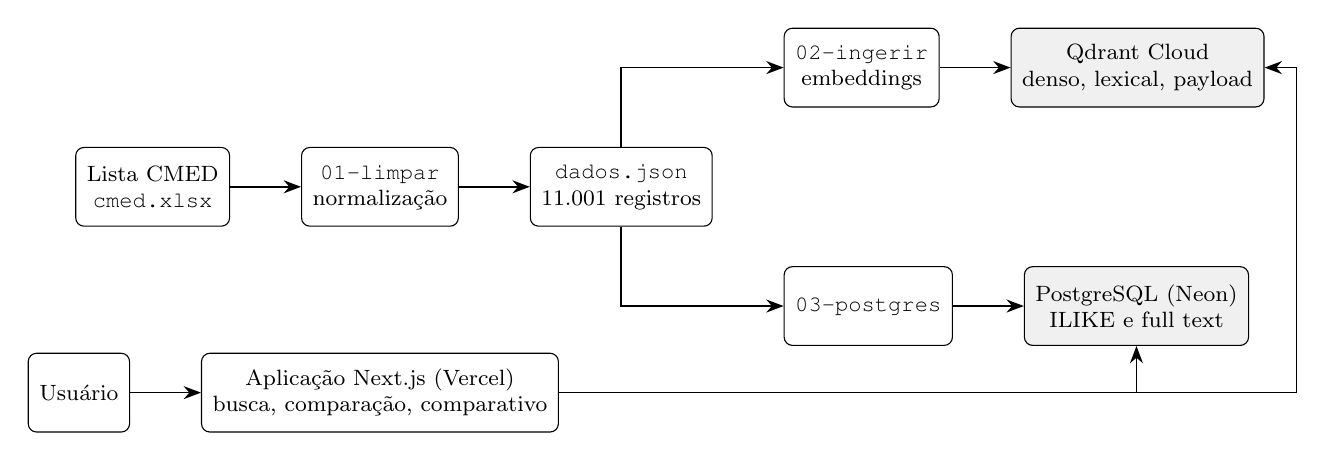
\begin{tikzpicture}[
      caixa/.style={draw, rounded corners=3pt, align=center, font=\footnotesize, minimum height=1.0cm, inner sep=4pt},
      seta/.style={-{Stealth[length=2.2mm]}, semithick},
      node distance=0.8cm and 0.9cm]
    \node[caixa] (xlsx) {Lista CMED\\\campo{cmed.xlsx}};
    \node[caixa, right=of xlsx] (limpar) {\campo{01-limpar}\\normalização};
    \node[caixa, right=of limpar] (json) {\campo{dados.json}\\11.001 registros};
    \node[caixa, above right=0.5cm and 0.9cm of json] (ingerir) {\campo{02-ingerir}\\embeddings};
    \node[caixa, below right=0.5cm and 0.9cm of json] (pg) {\campo{03-postgres}};
    \node[caixa, right=of ingerir, fill=black!6] (qdrant) {Qdrant Cloud\\denso, lexical, payload};
    \node[caixa, right=of pg, fill=black!6] (neon) {PostgreSQL (Neon)\\ILIKE e full text};
    \node[caixa, below=1.6cm of limpar, minimum width=4.2cm] (app) {Aplicação Next.js (Vercel)\\busca, comparação, comparativo};
    \node[caixa, left=of app] (usuario) {Usuário};
    \draw[seta] (xlsx) -- (limpar);
    \draw[seta] (limpar) -- (json);
    \draw[seta] (json) |- (ingerir);
    \draw[seta] (json) |- (pg);
    \draw[seta] (ingerir) -- (qdrant);
    \draw[seta] (pg) -- (neon);
    \draw[seta] (usuario) -- (app);
    % As setas da aplicação contornam as caixas por baixo e pela direita, sem cruzar o fluxo de carga.
    \draw[seta] (app.east) -| (neon.south);
    \draw[seta] (app.east) -| ([xshift=6mm]neon.east) |- (qdrant.east);
  \end{tikzpicture}}
  \fonte{Elaborada pelos autores.}
\end{figure}

\section{A base da CMED/ANVISA}

A fonte de dados é a Lista de Preços de Medicamentos da CMED, edição publicada em 09/10/2026 \cite{cmed2026}. O arquivo tem duas abas: ``Cabeçalho'', com notas explicativas, e ``Lista PMC'', com os dados, em 73 colunas e 26.635 registros. As colunas usadas estão na Tabela~\ref{tab:colunas}. As colunas de preço vêm em versões para cada alíquota de ICMS e o padrão adotado foi a de 19\%, aplicada em Goiás, configurável por variável de ambiente.

\begin{table}[htb]
  \centering
  \caption{Colunas da Lista PMC usadas no projeto}
  \label{tab:colunas}
  \footnotesize
  \begin{tabular}{|p{5.2cm}|p{8.8cm}|}
    \hline
    \textbf{Coluna} & \textbf{Uso} \\ \hline
    SUBSTÂNCIA & princípios ativos separados por ponto e vírgula \\ \hline
    PRODUTO, APRESENTAÇÃO & nome comercial; dosagem, forma e quantidade \\ \hline
    LABORATÓRIO, CNPJ & identificação do detentor do registro \\ \hline
    CÓDIGO GGREM, REGISTRO, EAN 1 & identificadores; o GGREM é único por apresentação \\ \hline
    CLASSE TERAPÊUTICA & código e descrição da classe (por exemplo, N2B2) \\ \hline
    TIPO DE PRODUTO (STATUS DO PRODUTO) & Genérico, Similar, Novo, Biológico, Específico e outros \\ \hline
    PMC 19 \%, PF 19 \% & preço máximo ao consumidor e preço fábrica com ICMS de 19\% \\ \hline
    RESTRIÇÃO HOSPITALAR & apresentações de uso restrito a hospitais \\ \hline
    COMERCIALIZAÇÃO 2025 & ``Sim'' quando o produto foi vendido em 2025 \\ \hline
    TARJA & Vermelha, Vermelha sob restrição, Preta, Sem Tarja, ``- (*)'' \\ \hline
  \end{tabular}
  \fonte{Elaborada pelos autores a partir de \citeonline{cmed2026}.}
\end{table}

\section{Limpeza e normalização dos dados}

O arquivo apresenta várias armadilhas, tratadas no script \campo{01-limpar.ts}. Os preços estão em texto com vírgula decimal (``27,22''); os campos vazios aparecem como um hífen cercado de espaços; os nomes das colunas de 0\% não seguem o mesmo padrão das demais (``PF 0\%'' e ``PMC 0 \%''); e a coluna DESTINAÇÃO COMERCIAL tem um espaço no fim do nome e está vazia em todas as linhas. O Código~\ref{cod:limpeza} mostra as funções de normalização de campos e números.

\begin{lstlisting}[language=TypeScript, caption={Normalização de campos vazios e números no padrão brasileiro}, label=cod:limpeza]
/** Campos vazios da planilha chegam como "    -     ". */
export function limparCampo(v: unknown): string | null {
  if (v === null || v === undefined) return null;
  const s = String(v).replace(/\s+/g, " ").trim();
  if (s === "" || s === "-") return null;
  return s;
}

/** "27,22", "1.250", "1.234,56", "1,0" */
export function numeroBR(v: unknown): number | null {
  const s = limparCampo(v);
  if (!s) return null;
  let t = s.replace(/[^\d.,]/g, "");
  if (t.includes(",")) t = t.replace(/\./g, "").replace(",", ".");
  else if (/^\d{1,3}(\.\d{3})+$/.test(t)) t = t.replace(/\./g, "");
  const n = Number(t);
  return Number.isFinite(n) ? n : null;
}
\end{lstlisting}

Foram descartados os registros não comercializados em 2025 e os sem PMC válido, a maior parte de uso hospitalar, cujo preço ao consumidor é omitido pela própria CMED. A Tabela~\ref{tab:limpeza} resume o resultado.

\begin{table}[htb]
  \centering
  \caption{Resultado da limpeza da Lista PMC}
  \label{tab:limpeza}
  \begin{tabular}{|l|r|}
    \hline
    \textbf{Etapa} & \textbf{Registros} \\ \hline
    Lidos da aba ``Lista PMC'' & 26.635 \\ \hline
    Descartados: COMERCIALIZAÇÃO 2025 = ``Não'' & 13.661 \\ \hline
    Descartados: sem PMC 19\% válido & 1.973 \\ \hline
    Registros finais & 11.001 \\ \hline
    Elegíveis para a busca (sem restrição hospitalar) & 10.996 \\ \hline
  \end{tabular}
  \fonte{Elaborada pelos autores.}
\end{table}

Da apresentação são extraídas a dosagem, a forma farmacêutica e a quantidade. A dosagem é normalizada para uma forma canônica, com os valores convertidos (``1 G'' passa a ``1000 MG'') e ordenados, para que ``35 MG + 300 MG + 50 MG'' e ``(35 + 300 + 50) MG'' gerem o mesmo resultado. As substâncias também recebem uma forma canônica, sem acento e sem descritores de hidratação (``anidra'', ``monoidratada''), mas preservando o sal: cloridrato e mucato de isometepteno continuam diferentes. Os registros finais se distribuem em 3.858 genéricos, 3.552 similares, 2.208 de referência, 719 específicos, 424 biológicos, 212 fitoterápicos e 28 sem tipo informado.

Algumas limitações vêm da própria fonte e foram mantidas como estão. A coluna de tipo não tem o valor ``Referência'': os produtos com tipo ``Novo'' recebem o selo de referência na interface, e 50 registros da lista bruta trazem apenas um hífen nessa coluna. O similar MIORRELAX aparece com ``citrato de orfenadrina'' como única substância, embora a apresentação informe três dosagens (300 mg, 50 mg e 35 mg), e por isso não entra no grupo de equivalência do Dorflex. Em 119 registros não foi possível extrair a dosagem, porque a apresentação não a informa (por exemplo, ``CAP MOLE CT BL AL AL X 30''), e em 82 não foi possível extrair a quantidade, o que impede o cálculo do preço por unidade nesses casos. A tarja ``- (*)'', que indica ausência da informação, foi convertida para ``Não informada''. Por fim, a fonte oficial não fornece imagens das embalagens: a ilustração exibida na interface é derivada apenas dos campos do registro, como descrito na Seção~\ref{sec:aplicacao}.

\section{Modelo de dados no Qdrant: collection, vetor e payload}

Os dados ficam em uma única collection chamada \campo{medicamentos}, com um ponto por apresentação e o identificador sequencial do registro como chave. Cada ponto tem três vetores nomeados, descritos na Tabela~\ref{tab:vetores}, e um \emph{payload} com os atributos do medicamento.

\begin{table}[htb]
  \centering
  \caption{Vetores nomeados da collection \campo{medicamentos}}
  \label{tab:vetores}
  \footnotesize
  \begin{tabular}{|p{2.3cm}|p{2.6cm}|p{9.0cm}|}
    \hline
    \textbf{Vetor} & \textbf{Tipo} & \textbf{Texto de origem} \\ \hline
    \campo{denso\_base} & denso, 384, cosseno & produto, substâncias, classe sem código, dosagem e forma por extenso; só dados da CMED (linha de base) \\ \hline
    \campo{denso} & denso, 384, cosseno & o mesmo texto acrescido dos termos populares do dicionário de indicações \\ \hline
    \campo{lexical} & esparso, modificador \campo{idf} & trigramas de caracteres de produto, substâncias e termos populares \\ \hline
  \end{tabular}
  \fonte{Elaborada pelos autores.}
\end{table}

O texto que vira vetor usa a forma farmacêutica por extenso (``comprimido revestido'' em vez de ``COM REV'') e omite os detalhes de embalagem (``CT BL AL PLAS''), que não ajudam a busca. O \emph{payload} guarda produto, substâncias (como lista), laboratório, apresentação, classe, tipo, selo, PMC, PF, registro, EAN, tarja, os indicadores de genérico e de restrição hospitalar, dosagem, forma, quantidade, preço por unidade e as chaves de equivalência. O Código~\ref{cod:collection} mostra a criação da collection.

\begin{lstlisting}[language=TypeScript, caption={Criação da collection com três vetores nomeados}, label=cod:collection]
await cliente.createCollection("medicamentos", {
  vectors: {
    denso_base: { size: 384, distance: "Cosine" },
    denso:      { size: 384, distance: "Cosine" },
  },
  sparse_vectors: { lexical: { modifier: "idf" } },
  hnsw_config: { m: 16, ef_construct: 128 },
});
\end{lstlisting}

\section{Índices de payload e chave de equivalência}

\begin{sloppypar}
Foram criados índices de \emph{payload} para os campos usados em filtros e agrupamentos: \campo{tipo\_produto}, \campo{selo}, \campo{tarja}, \campo{chave\_equivalencia} e \campo{chave\_equivalencia\_ampla} como palavras-chave; \campo{generico} e \campo{restricao\_hospitalar} como booleanos; e \campo{pmc} e \campo{preco\_por\_unidade} como números. Para os filtros de apresentação do site, foram acrescentados \campo{forma\_grupo} (o grupo da forma farmacêutica, como comprimido, cápsula ou gotas) e \campo{doses} (cada dose da apresentação na forma canônica) como palavras-chave, e \campo{quantidade\_num} como número. Com esses índices, o Qdrant aplica os filtros durante a busca no grafo, em vez de filtrar depois.
\end{sloppypar}

A equivalência entre apresentações usa duas chaves. A chave estrita junta as substâncias canônicas ordenadas, a dosagem canônica, a forma farmacêutica simplificada e a quantidade, por exemplo ``CAFEINA + CITRATO DE ORFENADRINA + DIPIRONA | 300 MG + 35 MG + 50 MG | COM | 24''; ela compara caixas iguais. A chave ampla é a mesma sem a quantidade e permite comparar caixas de tamanhos diferentes pelo preço por unidade, calculado como o PMC dividido pela quantidade. Na forma simplificada, drágea é tratada como comprimido e os qualificadores ``revestido'', ``dura'' e ``mole'' são ignorados, assim como o ``GEL'' de ``CAP GEL DURA'', que indica cápsula gelatinosa e não a forma gel. A quantidade conta os recipientes quando a apresentação os informa (``CT 6 SACH X 1G'' são 6 sachês, e não 1 g), e multiplica as unidades internas quando há uma contagem dentro de cada recipiente (``CT 25 STR X 10'' são 250 comprimidos). Essas duas regras foram corrigidas depois da publicação, a partir de casos apontados no uso do site: sem elas, o Floratil com 4 e com 6 sachês caíam no mesmo grupo, e o Repoflor em cápsula dura não encontrava o Floratil em cápsula gelatinosa de mesma dose. A correção alterou a chave de 622 registros e o texto vetorizado de 6, cujos vetores foram regerados; os resultados do benchmark do Capítulo~6 foram obtidos antes dela. Pela mesma via surgiram outras duas regras. A primeira trata como uma única forma o pó oral em envelope ou sachê descrito como ``PO OR'', ``PO LIOF'' ou ``PO PREP EXTEMP'', quando nada indica uso injetável e a forma não traz outro qualificador (como vaginal ou efervescente), e converte a dose por grama em dose por envelope (``200 MG/G'' em envelope de 1 g passa a 200 mg). A segunda é uma tabela de sinônimos de substâncias (\campo{data/sinonimos-substancias.json}), curada e versionada como o dicionário: a própria CMED registra produtos da mesma marca com nomes diferentes para o princípio ativo, como o Florent e o Repoflor, ora como ``LEVEDURA'', ora como ``SACCHAROMYCES BOULARDII'', e o Floralon com e sem a indicação da cepa (``- 17''). A tabela unifica esses nomes apenas na chave de equivalência, mantendo a exibição como na fonte, e cada entrada registra a evidência; a troca de ``LEVEDURA'' só vale quando ela é a única substância e a classe é a de antidiarreicos com microrganismos, para não alcançar associações como o Pantogar, em que a levedura é outro insumo. Para encontrar os demais casos de forma sistemática, foi criada uma auditoria automática (\campo{scripts/auditar-equivalencia.ts}, com relatório em \campo{docs/auditoria-equivalencia.md}). Ela lista marcas registradas com mais de um nome de substância, nomes que diferem só por espaço ou hífen, grupos com mesma substância, dose e quantidade separados apenas pela grafia da forma, e apresentações cuja leitura falhou. A partir dela, a tabela de sinônimos passou a 25 entradas, todas com uma marca registrada com os dois nomes como evidência (por exemplo, clorfenamina e clorfeniramina, mesalazina e messalazina, tiamazol e metimazol); os descritores de hidratação passaram a ser reconhecidos em qualquer grafia (``TRIHIDRATADA'', ``HEPTAIDRATADO''), o que juntou a amoxicilina com clavulanato do Clavulin aos genéricos; e as grafias da mesma forma foram unificadas (``CREM DERM'' e ``CREME'', ``SOL GOT OR'' e ``SOL OR'', ``SUS OC'' e ``SUS OFT''). Ficaram separados, de propósito, os sais diferentes (diclofenaco sódico, potássico e dietilamônio; ácido valproico e valproato de sódio) e as formas diferentes de verdade (comprimido e cápsula, creme e pomada, liberação imediata, prolongada, controlada e modificada, orodispersível, mastigável e efervescente). Com as regras atuais, a base tem 4.660 chaves estritas, das quais 1.558 agrupam dois ou mais registros e 1.340 contêm ao menos um genérico, e 3.082 chaves amplas, das quais 1.442 agrupam dois ou mais registros. No caso do Dorflex em caixa com 24 comprimidos, a chave estrita encontra apenas o similar Doricin, enquanto a chave ampla encontra 16 apresentações em outras caixas, como o Fenaflex e o Nevralgex.

Como decisão de modelagem, foi criado um dicionário de indicações em linguagem leiga (\campo{data/dicionario-indicacoes.json}), que associa termos populares a classes terapêuticas (``N2B2'': dor, febre, dor de cabeça) e a substâncias (fexofenadina: anti-histamínico de segunda geração, causa menos sonolência). A motivação está na Seção~\ref{sec:resultados-acuracia}: a base da CMED não diz para que serve cada medicamento em termos que o consumidor usa. O dicionário é conhecimento externo à fonte oficial e tem limitações declaradas: foi curado manualmente pelo grupo, cobre 84 classes, entre as mais frequentes no varejo, e 48 substâncias, não tem valor clínico e não traz indicação de uso nem dose. Com ele, 8.089 registros (73,5\%) receberam ao menos um termo popular. O mesmo texto enriquecido é usado no vetor denso e na base relacional, para que a comparação entre os bancos seja justa. A versão usada no benchmark (1.1) foi revisada inteira pelo critério de que cada termo deve ser defensável a partir da classe ou da substância, independentemente de qualquer consulta, e congelada antes da escrita das consultas, como descreve a Seção~\ref{sec:metodologia}.

% ---------------------------------------------------------------- 4
\chapter{Implementação}

\section{Instalação e configuração do Qdrant Cloud}

O Qdrant foi usado como serviço gerenciado no plano gratuito do Qdrant Cloud, com um cluster na região AWS de São Paulo. O acesso é feito pela URL do cluster e por uma chave de API, guardadas em variáveis de ambiente e nunca no código. A collection foi criada pelo próprio script de carga (Código~\ref{cod:collection}), seguida dos doze índices de \emph{payload}. Ao final da carga a collection ficou com 11.001 pontos, em dois segmentos e com status \campo{green}.

\section{Geração dos embeddings e carga}

Os embeddings são gerados pelo Transformers.js com o modelo quantizado em 8 bits, em lotes de 64 textos, e enviados ao Qdrant em lotes de 256 pontos. O módulo de embeddings fica atrás de uma interface única (\campo{ProvedorEmbeddings}), de modo que a troca por outro provedor afeta um único arquivo. A primeira carga, apenas com o vetor de linha de base, levou 592 s, sendo 479 s para gerar os embeddings na CPU e 112 s de envio. A carga final, com os três vetores, levou 652 s (619 s de embeddings e 30 s de envio) e reaproveitou os vetores da linha de base, guardados em arquivo, para não recalculá-los.

O vetor esparso é calculado sem vocabulário: cada trigrama de um alfabeto de 37 símbolos é convertido diretamente em um índice entre 0 e $37^3 - 1$ (Código~\ref{cod:trigramas}). O peso de cada trigrama no documento é $1/\sqrt{n}$, em que $n$ é o número de trigramas distintos do texto. Essa normalização foi introduzida depois que o primeiro teste mostrou vacinas, cujo campo de substância lista dezenas de sorotipos, aparecendo entre os primeiros resultados de quase qualquer consulta. Palavras vazias como ``de'', ``pra'' e ``que'' são descartadas, mas ``não'' é mantida de propósito.

\begin{lstlisting}[language=TypeScript, caption={Vetor esparso de trigramas de caracteres}, label=cod:trigramas]
const ALFABETO = " abcdefghijklmnopqrstuvwxyz0123456789";  // 37 símbolos

function trigramas(texto: string): number[] {
  const conjunto = new Set<number>();
  for (const palavra of normalizar(texto)) {          // sem acento e sem palavras vazias
    const p = ` ${palavra} `;
    for (let i = 0; i + 3 <= p.length; i++) conjunto.add(indiceTrigrama(p.slice(i, i + 3)));
  }
  return [...conjunto].sort((a, b) => a - b);
}

export function vetorTrigramasDocumento(texto: string) {
  const indices = trigramas(texto);
  const peso = 1 / Math.sqrt(indices.length || 1);    // evita que textos longos dominem
  return { indices, values: indices.map(() => peso) };
}
\end{lstlisting}

\section{Operações de consulta e filtragem}
\label{sec:consulta}

O site usa a busca híbrida. A consulta é transformada no vetor denso e no vetor esparso, e cada ramo recupera 50 candidatos com os mesmos filtros; o Qdrant funde as duas listas por \emph{Reciprocal Rank Fusion} \cite{cormack2009},
\begin{equation}
  \mathrm{RRF}(d) = \sum_{r \in R} \frac{1}{k + \mathrm{pos}_r(d)},
\end{equation}
em que $R$ é o conjunto de listas e $\mathrm{pos}_r(d)$ a posição do documento $d$ na lista $r$. A fusão usa só as posições, e não os escores, o que dispensa calibrar a escala do cosseno contra a do vetor esparso. Toda a operação é uma única chamada da Query API (Código~\ref{cod:hibrida}).

\begin{lstlisting}[language=JSON, caption={Corpo da consulta híbrida enviada à Query API}, label=cod:hibrida]
{
  "prefetch": [
    { "query": [0.031, -0.044, ...], "using": "denso", "limit": 50,
      "filter": { "must": [{ "key": "restricao_hospitalar", "match": { "value": false } }] },
      "params": { "hnsw_ef": 128 } },
    { "query": { "indices": [5214, 6033, ...], "values": [1, 1, ...] },
      "using": "lexical", "limit": 50, "filter": { ... } }
  ],
  "query": { "fusion": "rrf" },
  "limit": 22,
  "with_payload": ["produto", "substancia", "laboratorio", "pmc", "selo", ...]
}
\end{lstlisting}

Os filtros de somente genéricos, preço máximo, tarja, forma farmacêutica, dose e quantidade de unidades na caixa entram no campo \campo{filter} de cada ramo; a dose digitada pela pessoa (``75'', ``1 g'', ``500 mg/ml'') é convertida para a mesma forma canônica usada na base antes de virar filtro. A RRF produz empates exatos: os primeiros colocados de cada lista recebem o mesmo escore (no Qdrant, 0,5), e a ordem entre itens empatados não é garantida. Para que o resultado seja reprodutível, a aplicação busca alguns candidatos além do necessário e ordena por escore decrescente e, no empate, pelo identificador do ponto, um critério fixo e cego ao conteúdo. O mesmo desempate é aplicado aos outros motores, inclusive no \campo{ORDER BY} do PostgreSQL. A comparação de preços não usa vetores: recupera, por filtro exato sobre as chaves de equivalência, todos os pontos do grupo, e calcula a economia em relação ao medicamento escolhido.

\section{Reordenação dos resultados no site}
\label{sec:reordenacao}

Depois do benchmark, o uso do site revelou um problema na fusão por posições. Na consulta ``pregabalina 75 mg 30 cápsulas'', o ramo denso, que não conhece o nome do princípio ativo, colocou a furosemida em primeiro lugar, enquanto o ramo lexical acertou. Na RRF, os primeiros colocados dos dois ramos empatam, e a lista saiu intercalada entre pregabalina e medicamentos sem relação. Além disso, a dosagem e a quantidade digitadas não pesam em nenhum dos ramos. Para o site, foi criada uma reordenação leve, aplicada sobre a lista já fundida (\campo{lib/reordenacao.ts}). Ela lê o que a consulta pede de forma explícita e ordena por dois níveis: primeiro, os itens cujo nome de produto ou de princípio ativo contém uma palavra da consulta, ignorando nomes de sais, descritores químicos e formas farmacêuticas; depois, o número de itens de apresentação que coincidem (dosagem, quantidade, forma e o pedido de genérico). Dentro de cada nível vale a ordem da RRF. Quando a consulta não tem nome nem apresentação, como nas consultas coloquiais, a ordem não muda.

A regra do nome teve uma exceção, também encontrada no uso. A consulta ``febre'' trazia no topo as vacinas contra a febre amarela, porque a palavra aparece no nome do produto e da substância, embora ali designe a doença prevenida, e não um sintoma tratado. Quando a consulta usa uma palavra do dicionário de termos populares e nada mais do nome da vacina, as vacinas (classes terapêuticas J07 e J7) saem da lista; consultas como ``febre amarela'' e ``dengue'' continuam a encontrá-las. Uma regra mais geral, que deixasse de contar como nome qualquer palavra do dicionário, foi descartada porque erraria em produtos como colírios e o Espasmo Flatol, que trazem a palavra no nome e são o que a pessoa procura. A reordenação é usada só pelo site e pela API; o benchmark do Capítulo~6 mede o híbrido sem ela, e o efeito dela nas mesmas consultas é apresentado à parte na Seção~\ref{sec:vantagens}.

\section{A aplicação web}
\label{sec:aplicacao}

A aplicação foi construída com Next.js (App Router), TypeScript e Tailwind. A página inicial tem a logo e o campo de busca; os resultados aparecem em cartões com nome, laboratório, apresentação, preço, preço por unidade e selo, em páginas numeradas, com até 100 resultados por busca. Abaixo do campo de busca ficam os filtros de forma, dosagem e unidades na caixa, que começam sem preferência, e os demais (somente genéricos, preço máximo e tarja) ficam recolhidos. A busca usa formulário comum, sem depender de JavaScript, e o endereço da página de resultados pode ser compartilhado. O percentual de similaridade de cosseno foi deliberadamente deixado fora dos cartões: ao lado de um preço, um número como ``52\%'' tende a ser lido como desconto. Ele aparece apenas na página de comparativo, identificado como ``52\% de similaridade'', onde a métrica faz sentido. Ao clicar em um cartão, a página de comparação mostra os equivalentes da mesma caixa, do mais barato ao mais caro, e, abaixo, os equivalentes em caixas de outro tamanho ordenados pelo preço por unidade, com a diferença de cada equivalente em relação ao escolhido (``58\% mais barato''). A comparação é apresentada em porcentagem, e não em reais, por uma razão dos próprios dados: o PMC é um teto legal e o Preço Fábrica é uma fração quase fixa dele (mediana de 72,5\% na base), de modo que nenhum dos dois corresponde ao preço praticado no balcão. Em um teste informal, um usuário relatou ter pago por dois medicamentos menos do que o próprio Preço Fábrica (66\% e 76\% dele). A diferença relativa entre equivalentes é a informação mais confiável que a base oferece; o teto aparece em letra menor, como ``Preço máximo: até R\$ X'', com a explicação de que a farmácia não pode cobrar mais e costuma cobrar menos. A página de comparativo executa a mesma consulta nos cinco motores, mostra os tempos e, para as consultas do benchmark, marca cada resultado pelo gabarito. Um rodapé fixo informa que os valores são o teto da CMED e que a ferramenta não substitui orientação médica ou farmacêutica.

Como a fonte não fornece imagens, cada apresentação é ilustrada por um SVG gerado a partir do próprio registro, em estilo de caixa de medicamento. A ilustração é um retângulo simples na cor da marca, com o nome do produto em destaque, a dosagem, o princípio ativo, o conteúdo por extenso (``Contém 20 comprimidos revestidos'') e a via de uso deduzida da forma farmacêutica (``USO ORAL''), além de um ícone branco da forma no canto, com o nome dela embaixo (comprimido, cápsula, gotas, xarope, creme, injetável). Quando o registro informa tarja vermelha ou preta, aparece a faixa correspondente com a frase de venda (``VENDA SOB PRESCRIÇÃO MÉDICA'' e, nos casos de retenção, ``SÓ PODE SER VENDIDO COM RETENÇÃO DA RECEITA''). Nos genéricos, a parte inferior traz a faixa amarela com a letra ``G'' e a menção à Lei nº 9.787/1999, que é a identificação obrigatória desses medicamentos; os demais tipos não recebem faixa, como nas caixas reais, e o tipo aparece num selo ao lado da ilustração. A cor sai de uma paleta fixa, escolhida por um \emph{hash} do nome da marca; nos genéricos, do laboratório, que costuma usar a mesma cor em toda a linha. O laboratório aparece apenas como texto, sem logotipo nem identidade visual de nenhum fabricante.

A publicação na Vercel trouxe uma consequência prática da escolha do modelo local. A função que gera os embeddings precisa levar o modelo (113 MB do arquivo ONNX e 16 MB do vocabulário) e o binário nativo do onnxruntime para Linux, de 44 MB, perto do limite de 250 MB por função. O rastreador de dependências do Next.js não detectava o binário, carregado dinamicamente, e incluía por engano um cache do modelo; por isso o modelo passou a ser baixado durante o build e incluído explicitamente, junto apenas com o binário para Linux x64. Pelo rastreamento do Next.js, a função ficou com 193 MB; na contagem da Vercel, que considera o pacote descompactado na plataforma, com 342 MB. A alternativa prevista, caso o limite fosse ultrapassado, era trocar o onnxruntime nativo pela versão WebAssembly, mantendo o modelo local, sem chave de API e sem custo; ela não foi necessária. Duas outras restrições apareceram: o plano gratuito aceita no máximo 12 funções por publicação, o que obrigou a restringir o modelo às rotas de busca (e, depois, a uma única rota, por causa do armazenamento; ver Seção~\ref{sec:vantagens}), e a região padrão das funções ficava nos Estados Unidos, longe dos bancos, e foi fixada em São Paulo. Em produção, a primeira requisição após a criação de uma instância levou 3,7 s, dos quais 2,26 s para carregar o modelo; com a instância ativa, o processamento dentro da função ficou entre 25 e 120 ms.

% ---------------------------------------------------------------- 5
\chapter{Abordagem relacional equivalente}

\section{Modelagem no PostgreSQL}

A base relacional foi criada no Neon, um PostgreSQL gerenciado gratuito, na mesma região dos demais serviços. Uma única tabela, \campo{medicamentos}, guarda os mesmos 11.001 registros com as mesmas colunas do \emph{payload} e os textos de indexação, inclusive o texto enriquecido pelo dicionário. Foram usadas as extensões \campo{unaccent}, para comparar sem acentos, e \campo{pg\_trgm}, para indexar buscas por substring \cite{pgtrgm}. Como a função \campo{unaccent} não é imutável, ela foi encapsulada numa função \campo{IMMUTABLE} para poder ser usada em índices. Uma configuração de busca textual derivada da portuguesa aplica o \emph{stemmer} e remove acentos. O vetor de busca é uma coluna gerada com pesos por campo (Código~\ref{cod:ddl}). A carga levou 3,2 s, ou 3,8 s com a criação dos índices, e a tabela ocupa 17 MB com eles.

\begin{lstlisting}[language=SQL, caption={Configuração em português sem acentos e coluna de busca com pesos}, label=cod:ddl]
CREATE TEXT SEARCH CONFIGURATION pt_unaccent (COPY = portuguese);
ALTER TEXT SEARCH CONFIGURATION pt_unaccent
  ALTER MAPPING FOR hword, hword_part, word WITH unaccent, portuguese_stem;

ALTER TABLE medicamentos ADD COLUMN busca tsvector GENERATED ALWAYS AS (
  setweight(to_tsvector('pt_unaccent', produto), 'A') ||
  setweight(to_tsvector('pt_unaccent', f_juntar(substancia)), 'B') ||
  setweight(to_tsvector('pt_unaccent', texto_enriquecido), 'C')
) STORED;

CREATE INDEX medicamentos_busca_gin  ON medicamentos USING gin (busca);
CREATE INDEX medicamentos_texto_trgm ON medicamentos
  USING gin (f_unaccent(lower(texto_enriquecido)) gin_trgm_ops);
\end{lstlisting}

\section{Busca com ILIKE}

A busca por \campo{ILIKE} representa a abordagem mais comum em aplicações simples: cada palavra da consulta, sem acento e em minúsculas, precisa aparecer como substring do texto enriquecido. Nenhuma palavra é descartada, o que corresponde a uma busca literal. Como \campo{ILIKE} não produz um escore de relevância, os resultados são ordenados com prioridade para produtos cujo nome começa pela primeira palavra da consulta, depois por nomes mais curtos e pelo preço (Código~\ref{cod:ilike}). O índice de trigramas acelera o filtro por substring.

\begin{lstlisting}[language=SQL, caption={Consulta por ILIKE}, label=cod:ilike]
SELECT id, produto, substancia, laboratorio, pmc, selo, ...
FROM medicamentos
WHERE f_unaccent(lower(texto_enriquecido)) LIKE ALL($1::text[])  -- '%palavra%' por palavra
  AND NOT restricao_hospitalar
ORDER BY (f_unaccent(lower(produto)) LIKE $2) DESC, length(produto), pmc, id
LIMIT 10;
\end{lstlisting}

\section{Busca com full text search em português}

A busca textual completa usa \campo{websearch\_to\_tsquery} na configuração em português, que remove palavras vazias e reduz as palavras ao radical, e ordena os resultados por \campo{ts\_rank\_cd}, que considera os pesos dos campos e a proximidade entre os termos \cite{pgfts}. A consulta exige todos os termos, com E lógico. Quando nada é encontrado, o que ocorre com frequência em consultas coloquiais, a consulta é refeita com OU entre os radicais (Código~\ref{cod:fts}). Esse relaxamento é uma prática comum e foi adotado para não subestimar a abordagem relacional.

\begin{lstlisting}[language=SQL, caption={Busca textual completa com relaxamento de E para OU}, label=cod:fts]
-- 1a tentativa: todos os termos
WITH q AS (SELECT websearch_to_tsquery('pt_unaccent', $1) AS tq)
SELECT ..., ts_rank_cd(busca, q.tq) AS rank FROM medicamentos, q
WHERE busca @@ q.tq AND NOT restricao_hospitalar
ORDER BY rank DESC, pmc, id LIMIT 10;

-- se não houver resultado: OU entre os radicais da consulta
WITH q AS (SELECT to_tsquery('pt_unaccent', string_agg(lexeme, ' | '))
           FROM unnest(to_tsvector('pt_unaccent', $1)))
...
\end{lstlisting}

% ---------------------------------------------------------------- 6
\chapter{Análise comparativa}

\section{Metodologia do experimento}
\label{sec:metodologia}

Foram comparados cinco motores sobre os mesmos 11.001 registros: denso sem enriquecimento (vetor \campo{denso\_base}, linha de base), denso com enriquecimento (vetor \campo{denso}), híbrido (denso enriquecido e esparso fundidos por RRF), \campo{ILIKE} e busca textual completa. Os três primeiros rodam no Qdrant e os dois últimos no PostgreSQL. Em todos, a busca retorna os dez primeiros resultados, com o filtro padrão do site, que oculta as apresentações de uso hospitalar.

\textbf{Protocolo contra vazamento.} Durante o desenvolvimento, três consultas foram usadas para diagnosticar a busca densa pura: ``dorflex'', ``remédio pra dor de cabeça'' e ``antialérgico que não dá sono''. A primeira versão do dicionário continha literalmente a frase ``antialérgico que não dá sono'', o que fazia o \campo{ILIKE} e a busca textual acertarem essa consulta por casamento exato de palavras. O vazamento foi corrigido, e não apenas declarado: o dicionário foi revisado inteiro pelo critério de que cada termo deve ser defensável a partir da classe ou da substância. Nessa revisão saíram as frases sobre sono escritas com a consulta em mente, os termos ``dor de cabeça'' e ``enxaqueca'' da classe A3D, que só se justificam pela substância isometepteno, e ``remédio para dormir'' da classe N5B1. O protocolo adotado a partir daí tem quatro regras:
\begin{enumerate}
  \item o dicionário foi congelado no commit \texttt{\seqsplit{aa9df017a8c8d01a8bef3d2adc72ea9e72c5402f}} (versão 1.1), antes de as consultas de teste serem escritas;
  \item as consultas foram escritas depois desse commit, no commit \campo{62a2101}, e ajustadas uma única vez antes da primeira execução, no commit \campo{7bb7ed7};
  \item as consultas de teste não foram usadas para ajustar o dicionário nem os motores;
  \item as três consultas originais permanecem no conjunto, marcadas como usadas durante o desenvolvimento, e os resultados são apresentados com e sem elas.
\end{enumerate}
Seguindo o mesmo princípio, outras consultas usadas em testes durante o ajuste da camada lexical (``dipirna'', ``neosaudina'', ``paracetamol 750'' e ``tylenol'') ficaram fora do conjunto de teste. Também foi uma decisão metodológica não aumentar o peso do nome comercial no vetor esparso: o teste com peso maior foi feito com as consultas de desenvolvimento, piorou as consultas coloquiais, e continuar ajustando o motor sobre consultas que estariam no conjunto de teste enviesaria o resultado a favor do híbrido.

\textbf{Métricas.} Para cada consulta, um resultado é correto quando atende ao gabarito, definido por princípio ativo, classe terapêutica ou combinação deles (Seção~\ref{sec:consultas}). As métricas seguem as definições usuais de recuperação de informação \cite{manning2008}: acerto no top 5 (proporção de consultas com pelo menos um resultado correto entre os cinco primeiros); MRR@10, a média do inverso da posição do primeiro resultado correto entre os dez primeiros, valendo zero quando não há acerto; precisão no top 5, a proporção de resultados corretos entre os cinco primeiros, contando posições vazias como incorretas; posição média do primeiro resultado correto, calculada só nas consultas em que ele aparece; e número de consultas sem acerto no top 10.

\textbf{Dificuldade.} Os gabaritos variam de 8 a 985 registros válidos, de modo que as consultas não têm a mesma dificuldade. Para cada consulta foi calculada a probabilidade de um motor que sorteasse cinco resultados ao acaso acertar ao menos um,
\begin{equation}
  p_{\text{acaso}} = 1 - \binom{N - K}{5} \Big/ \binom{N}{5},
\end{equation}
em que $N = 10.996$ é o número de registros elegíveis e $K$ o número de registros válidos para o gabarito. O acerto ponderado dá a cada consulta o peso $1 - p_{\text{acaso}}$, de modo que uma consulta com gabarito amplo, em que qualquer motor acerta, vale menos que uma consulta difícil.

\textbf{Procedimento de medição.} O plano gratuito do Neon suspende o servidor quando ocioso, e a primeira consulta depois disso leva segundos. O Qdrant e o modelo de embeddings também têm custo de primeira chamada. Por isso, antes de medir, cada motor recebe cinco consultas genéricas e, em seguida, uma passada completa pelas 28 consultas do conjunto, todas descartadas. Cada consulta é então executada cinco vezes por motor, alternando os motores, e o tempo reportado é a mediana. São registrados três tempos: o do embedding da consulta, o do banco ponta a ponta, medido no cliente e incluindo a rede, e o do banco no servidor, que é o campo \campo{time} da resposta do Qdrant e o tempo de planejamento mais execução do \campo{EXPLAIN ANALYZE} no PostgreSQL. Os dois bancos devolvem o mesmo conjunto reduzido de campos, apenas os exibidos na interface.

Esse procedimento é resultado de duas revisões, resumidas na Tabela~\ref{tab:revisoes}. Na primeira execução o aquecimento tinha apenas as cinco consultas genéricas, e o cache frio do vetor denso, recém-gravado, deixou as primeiras consultas do denso enriquecido e do híbrido entre 70 e 85 ms, inflando o percentil 95. Ao repetir a medição com aquecimento completo, apareceu uma diferença de acurácia que não deveria existir: 18 medições do híbrido mudaram de posição entre execuções, por causa dos empates exatos da RRF. Com o desempate fixo descrito na Seção~\ref{sec:consulta}, uma verificação com execuções repetidas confirmou que os cinco motores passaram a devolver exatamente o mesmo top 10. Por fim, o tempo ponta a ponta do Qdrant mostrou um padrão de ``30 ou 70 ms'' que não dependia do motor: respostas acima de cerca de 1,5 KB ganhavam um atraso fixo de cerca de 40 ms no cliente, característico da interação entre o algoritmo de Nagle e o reconhecimento atrasado do TCP \cite{rfc896,rfc1122}, enquanto o próprio Qdrant gastava menos de 2 ms. A medição passou então a registrar também o tempo no servidor. Todos os números deste capítulo são da execução final, que se reproduz.

\begin{table}[htb]
  \centering
  \caption{Revisões do procedimento de medição}
  \label{tab:revisoes}
  \footnotesize
  \begin{tabular}{|p{1.9cm}|p{5.6cm}|p{6.3cm}|}
    \hline
    \textbf{Execução} & \textbf{Problema observado} & \textbf{Correção} \\ \hline
    1ª & cache frio do vetor recém-gravado inflava o p95 do denso enriquecido e do híbrido & aquecimento com uma passada completa descartada por motor \\ \hline
    2ª & 18 medições do híbrido mudavam de posição entre execuções (empates da RRF) & desempate fixo por identificador em todos os motores; verificação de determinismo \\ \hline
    3ª & tempo ponta a ponta do Qdrant com +40 ms em respostas maiores (Nagle e ACK atrasado) & registro do tempo no servidor; mesmo conjunto reduzido de campos nos dois bancos \\ \hline
    Final & acurácia idêntica à da 3ª execução & resultados usados neste relatório \\ \hline
  \end{tabular}
  \fonte{Elaborada pelos autores.}
\end{table}

\section{Conjunto de consultas de teste}
\label{sec:consultas}

O conjunto tem 28 consultas (Tabela~\ref{tab:consultas}): 5 por nome comercial, 5 com erro de digitação, 1 de variação de nomenclatura, 5 por princípio ativo, 9 em linguagem coloquial e 3 mistas. As consultas coloquiais novas são paráfrases que não aparecem no dicionário. A consulta ``simvastatina'' foi inicialmente classificada como erro de digitação, mas corresponde à grafia internacional do princípio ativo; foi reclassificada como variação de nomenclatura antes da primeira execução, e ``nimezulida'' foi incluída para manter cinco erros de digitação reais. Excluindo as três consultas de desenvolvimento, restam 25.

Um verificador confere, sem executar nenhum motor, se o gabarito de cada consulta tem registros válidos na base e se a consulta aparece no dicionário ou contém um termo composto dele. Nenhuma das consultas novas foi sinalizada. A coincidência de palavras isoladas, porém, é inevitável: ``alergia'' e ``sonolência'' na consulta 16, ``queimação'' e ``estômago'' na 19 e ``anti-inflamatório'' na 23, por exemplo, são palavras de termos do dicionário. Em vez de tentar eliminá-la, essa sobreposição foi medida (coluna ``Coinc.'' da Tabela~\ref{tab:consultas}). Ela favorece o \campo{ILIKE} e a busca textual nessas consultas, como discutido na Seção~\ref{sec:vantagens}.

\begin{table}[p]
  \centering
  \caption{Consultas de teste, gabarito e dificuldade}
  \label{tab:consultas}
  \scriptsize
  \setlength{\tabcolsep}{4pt}
  \begin{tabular}{|r|p{1.9cm}|p{3.7cm}|p{5.2cm}|r|r|r|}
    \hline
    \textbf{Nº} & \textbf{Categoria} & \textbf{Consulta} & \textbf{Correto quando} & \textbf{K} & \textbf{$p$ (\%)} & \textbf{Coinc.} \\ \hline
    1* & nome comercial & dorflex & DORFLEX ou dipirona + orfenadrina + cafeína & 24 & 1,1 & 0 \\ \hline
    2 & nome comercial & allegra & ALLEGRA ou fexofenadina isolada & 44 & 2,0 & 0 \\ \hline
    3 & nome comercial & buscopan & BUSCOPAN ou escopolamina isolada & 8 & 0,4 & 0 \\ \hline
    4 & nome comercial & novalgina & NOVALGINA ou dipirona isolada & 111 & 4,9 & 0 \\ \hline
    5 & nome comercial & puran t4 & PURAN T4 ou levotiroxina isolada & 63 & 2,8 & 0 \\ \hline
    6 & erro de digitação & loratadna & loratadina (desloratadina não conta) & 36 & 1,6 & 0 \\ \hline
    7 & erro de digitação & omeprasol & omeprazol & 59 & 2,7 & 0 \\ \hline
    8 & erro de digitação & amoxilina & amoxicilina, isolada ou associada & 161 & 7,1 & 0 \\ \hline
    9 & erro de digitação & iboprofeno & ibuprofeno & 127 & 5,6 & 0 \\ \hline
    28 & erro de digitação & nimezulida & nimesulida & 48 & 2,2 & 0 \\ \hline
    10 & variação de nomenclatura & simvastatina & sinvastatina & 64 & 2,9 & 0 \\ \hline
    11 & princípio ativo & losartana 50 mg & losartana com 50 mg & 43 & 1,9 & 0 \\ \hline
    12 & princípio ativo & atorvastatina & atorvastatina & 53 & 2,4 & 0 \\ \hline
    13 & princípio ativo & cloridrato de sertralina & sertralina & 50 & 2,3 & 0 \\ \hline
    14 & princípio ativo & amoxicilina com clavulanato & exatamente amoxicilina + clavulanato & 77 & 3,5 & 0 \\ \hline
    15 & princípio ativo & metformina 850 & metformina com 850 mg & 26 & 1,2 & 0 \\ \hline
    16 & coloquial & alergia sem sonolência & anti-histamínico de segunda geração & 166 & 7,3 & 2 \\ \hline
    17 & coloquial & cabeça latejando & analgésico, antitérmico ou antienxaqueca & 707 & 28,3 & 1 \\ \hline
    18 & coloquial & costas travadas de tanto pegar peso & relaxante muscular ou anti-inflamatório & 591 & 24,1 & 2 \\ \hline
    19 & coloquial & queimação no estômago depois de comer & antiácido ou inibidor de acidez & 315 & 13,5 & 2 \\ \hline
    20 & coloquial & nariz escorrendo e espirrando o tempo todo & anti-histamínico, antigripal ou preparação nasal & 380 & 16,1 & 1 \\ \hline
    21 & coloquial & intestino travado há dias & laxante & 63 & 2,8 & 1 \\ \hline
    22 & coloquial & pressão sempre lá em cima & anti-hipertensivo & 985 & 37,5 & 1 \\ \hline
    26* & coloquial & remédio pra dor de cabeça & mesmo critério da 17 & 707 & 28,3 & 2 \\ \hline
    27* & coloquial & antialérgico que não dá sono & mesmo critério da 16 & 166 & 7,3 & 1 \\ \hline
    23 & mista & anti-inflamatório barato genérico & anti-inflamatório não esteroidal e genérico & 159 & 7,0 & 1 \\ \hline
    24 & mista & dipirona gotas genérico & dipirona isolada, genérica, em solução oral & 23 & 1,0 & 0 \\ \hline
    25 & mista & xarope pra tosse carregada & expectorante em xarope & 174 & 7,7 & 2 \\ \hline
  \end{tabular}
  \fonte{Elaborada pelos autores a partir de \campo{benchmark/consultas.json}.}
  \nota{* consulta usada durante o desenvolvimento. K = registros válidos entre os 10.996 elegíveis; $p$ = probabilidade de acerto no top 5 ao acaso; Coinc. = palavras da consulta que coincidem com palavras do dicionário.}
\end{table}

\section{Resultados de acurácia}
\label{sec:resultados-acuracia}

A Tabela~\ref{tab:acuracia} e a Figura~\ref{fig:acerto} apresentam os resultados. O híbrido teve o maior acerto no top 5 (80\% nas 25 consultas novas), seguido pela busca textual (68\%). O acerto ponderado pela dificuldade praticamente não altera a ordem nem os valores, o que indica que as diferenças não vêm de consultas fáceis. A média de acerto ao acaso foi de 7,6\%. A inclusão das três consultas de desenvolvimento muda os valores em no máximo três pontos percentuais.

\begin{table}[htb]
  \centering
  \caption{Acurácia dos cinco motores}
  \label{tab:acuracia}
  \scriptsize
  \setlength{\tabcolsep}{4pt}
  \begin{tabular}{|l|c|c|c|c|c|c|}
    \hline
    \textbf{Motor} & \textbf{Acerto top 5} & \textbf{Ponderado} & \textbf{MRR@10} & \textbf{Precisão top 5} & \textbf{Posição média} & \textbf{Sem acerto} \\ \hline
    Denso sem enriquecimento & 28\% (29\%) & 27\% (27\%) & 0,17 (0,17) & 0,16 (0,15) & 3,3 (3,8) & 17 (18) \\ \hline
    Denso com enriquecimento & 40\% (43\%) & 38\% (41\%) & 0,29 (0,33) & 0,25 (0,29) & 2,0 (1,8) & 15 (16) \\ \hline
    Híbrido (RRF) & 80\% (82\%) & 80\% (82\%) & 0,66 (0,69) & 0,42 (0,46) & 2,4 (2,2) & 2 (2) \\ \hline
    ILIKE & 36\% (36\%) & 38\% (38\%) & 0,36 (0,36) & 0,35 (0,35) & 1,0 (1,0) & 16 (18) \\ \hline
    Full text & 68\% (68\%) & 67\% (67\%) & 0,65 (0,63) & 0,64 (0,63) & 1,4 (1,4) & 7 (8) \\ \hline
  \end{tabular}
  \fonte{Elaborada pelos autores a partir de \campo{benchmark/resultados.json}.}
  \nota{Valores das 25 consultas novas; entre parênteses, com as 3 de desenvolvimento (28 consultas). ``Sem acerto'' conta as consultas sem resultado correto no top 10.}
\end{table}

\begin{figure}[htb]
  \centering
  \caption{Acerto no top 5 por motor, simples e ponderado pela dificuldade}
  \label{fig:acerto}
  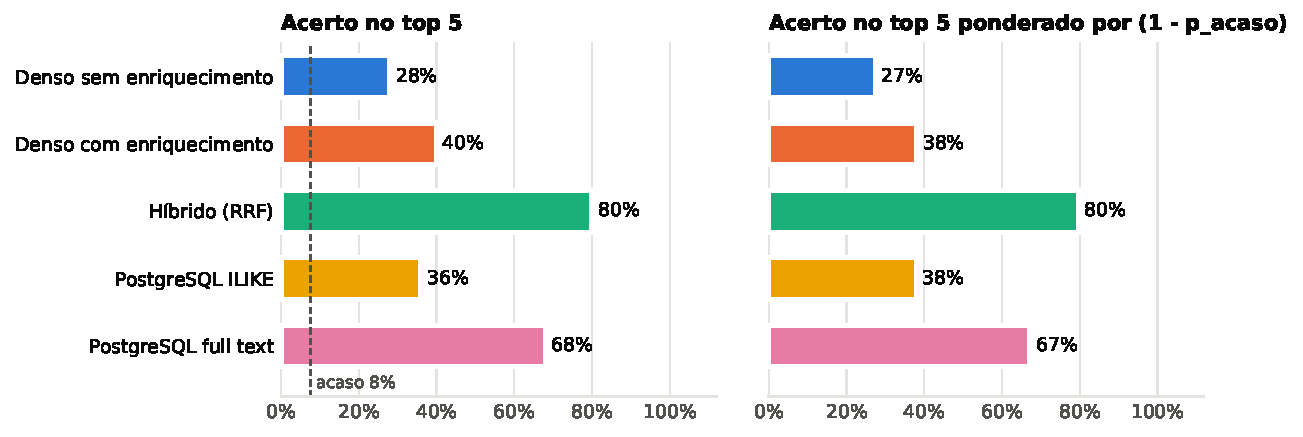
\includegraphics[width=\textwidth]{figuras/fig1-acerto-por-motor.pdf}
  \fonte{Elaborada pelos autores. A linha tracejada indica o acerto médio ao acaso.}
\end{figure}

A evolução da busca vetorial é o resultado mais interessante do experimento (Tabela~\ref{tab:evolucao} e Figura~\ref{fig:evolucao}). O vetor denso sem enriquecimento acertou 28\% das consultas e não encontrou nenhum resultado correto no top 10 em 17 das 25. Na consulta ``dorflex'', os cinco primeiros resultados foram Doxuran, Doxiclin e Dobutrex: o modelo quebra o nome comercial em pedaços e aproxima nomes de grafia parecida, sem relação terapêutica. O enriquecimento com termos populares elevou o acerto para 40\% e resolveu boa parte das consultas coloquiais, porque o texto do Dorflex passou a conter ``relaxante muscular, dor''. A busca híbrida dobrou o acerto, para 80\%, e reduziu de 15 para 2 as consultas sem acerto: o vetor esparso recupera nomes comerciais e erros de digitação, que o vetor denso não representa bem.

\begin{table}[htb]
  \centering
  \caption{Evolução da busca vetorial: antes e depois do enriquecimento e da busca híbrida}
  \label{tab:evolucao}
  \footnotesize
  \begin{tabular}{|p{4.2cm}|p{3.0cm}|p{3.0cm}|p{3.0cm}|}
    \hline
    & \textbf{Denso sem enriquecimento} & \textbf{Denso com enriquecimento} & \textbf{Híbrido (RRF)} \\ \hline
    Acerto no top 5 & 28\% & 40\% & 80\% \\ \hline
    Acerto ponderado & 27\% & 38\% & 80\% \\ \hline
    MRR@10 & 0,17 & 0,29 & 0,66 \\ \hline
    Consultas sem acerto no top 10 & 17 & 15 & 2 \\ \hline
    1º resultado para ``dorflex'' & Doxuran (doxazosina) & Doricin (equivalente) & Doricin (equivalente) \\ \hline
    1º resultado para ``remédio pra dor de cabeça'' & Vertigium (flunarizina) & Maxalgina (dipirona) & Maxalgina (dipirona) \\ \hline
    1º resultado para ``antialérgico que não dá sono'' & Dormec (ácido acetilsalicílico) & Dormonid (midazolam) & Naire (bilastina) \\ \hline
  \end{tabular}
  \fonte{Elaborada pelos autores. As métricas são das 25 consultas novas; as três linhas finais são as consultas usadas durante o desenvolvimento.}
\end{table}

\begin{figure}[htb]
  \centering
  \caption{Evolução da busca vetorial}
  \label{fig:evolucao}
  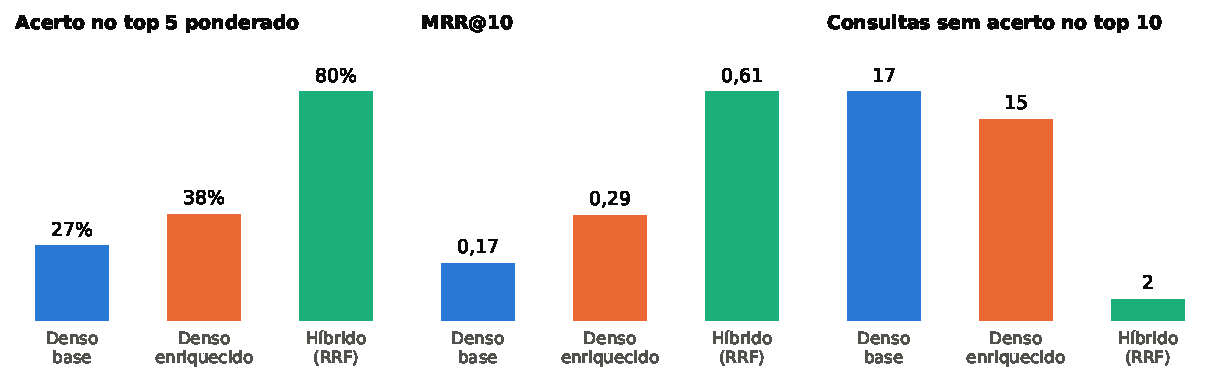
\includegraphics[width=\textwidth]{figuras/fig2-evolucao-vetorial.pdf}
  \fonte{Elaborada pelos autores a partir das 25 consultas novas.}
\end{figure}

Por categoria (Figura~\ref{fig:categoria}), cada abordagem vence em uma frente. O \campo{ILIKE} e a busca textual acertam todas as consultas por nome comercial e por princípio ativo, em que basta o casamento literal, e nenhuma com erro de digitação. Os motores densos fazem o oposto: acertam 60\% dos erros de digitação e quase nenhuma consulta de uma única palavra rara, como ``allegra'' e ``atorvastatina'', cujo vetor fica próximo de ruído e devolve vacinas e toxina botulínica. O híbrido é o único que vai bem nas duas frentes, com 80\% a 100\% em nome comercial, erro de digitação e princípio ativo. Nas consultas coloquiais, a busca textual empata com o híbrido (86\%). Nenhum motor acertou ``simvastatina'' nem ``loratadna'' (Figura~\ref{fig:posicoes}).

\begin{figure}[htb]
  \centering
  \caption{Acerto no top 5 por categoria e motor}
  \label{fig:categoria}
  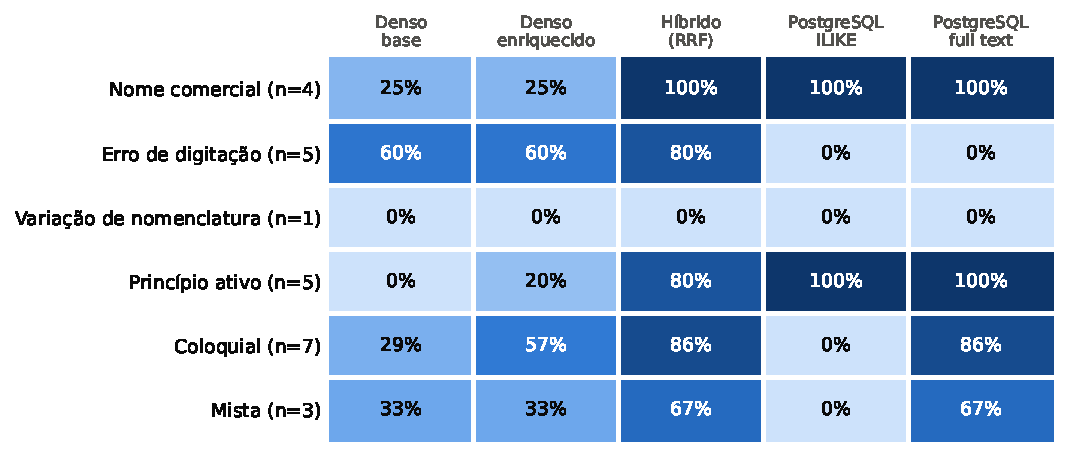
\includegraphics[width=0.92\textwidth]{figuras/fig3-acerto-por-categoria.pdf}
  \fonte{Elaborada pelos autores a partir das 25 consultas novas.}
\end{figure}

\begin{figure}[p]
  \centering
  \caption{Posição do primeiro resultado correto, por consulta e motor}
  \label{fig:posicoes}
  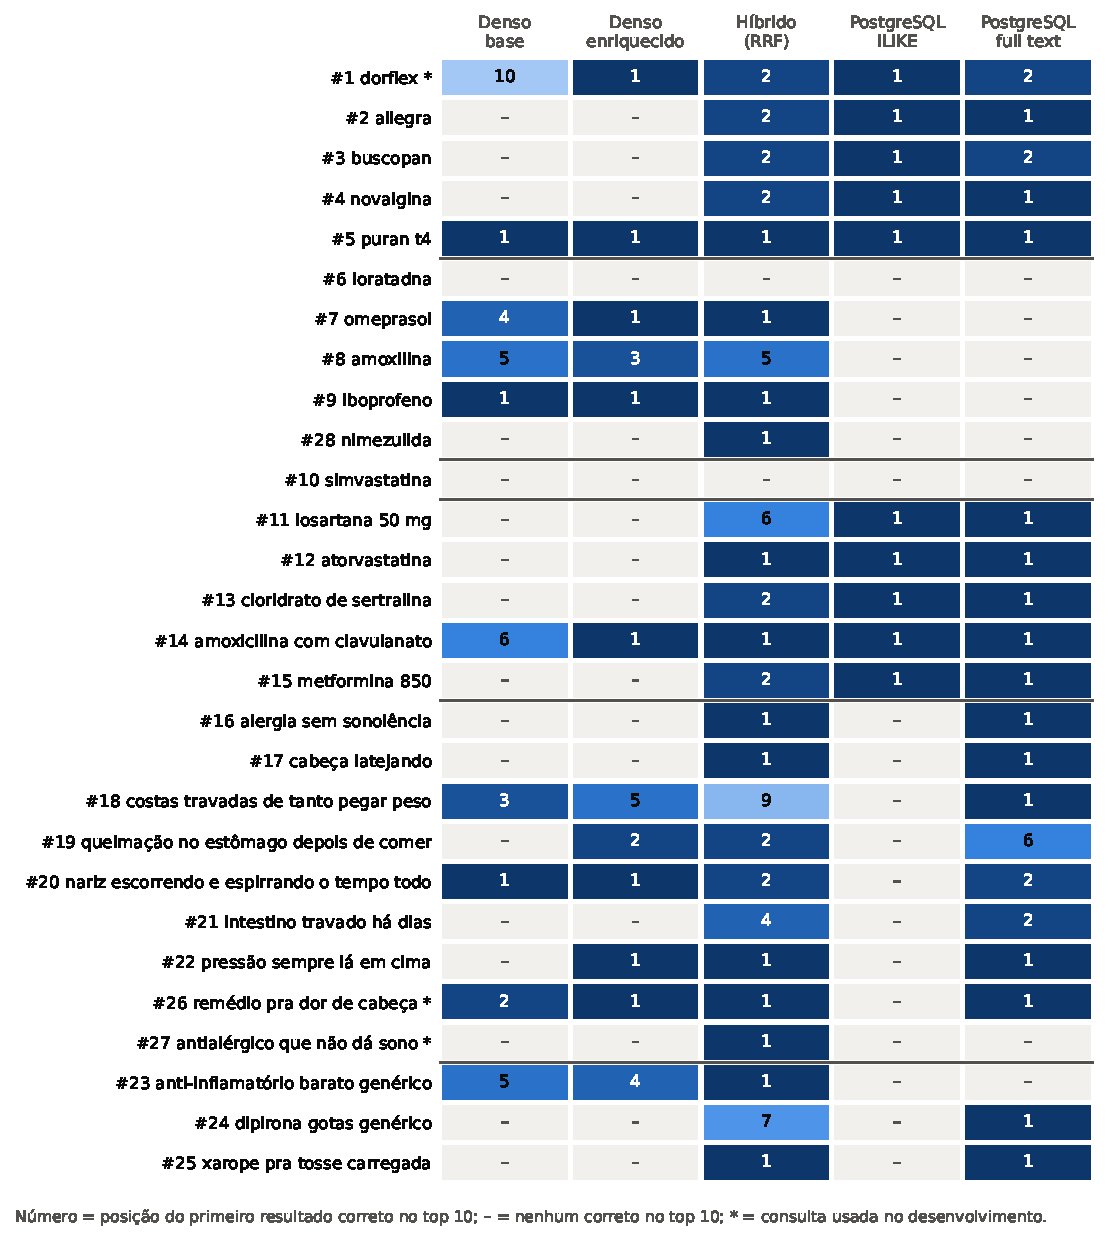
\includegraphics[height=0.82\textheight,width=\textwidth,keepaspectratio]{figuras/fig5-posicao-por-consulta.pdf}
  \fonte{Elaborada pelos autores a partir de \campo{benchmark/resultados.json}.}
\end{figure}

\section{Limitação da negação}

As consultas que pedem um antialérgico que não cause sono mostram uma limitação das três abordagens, que merece ser tratada à parte. A Tabela~\ref{tab:negacao} mostra os cinco primeiros resultados de cada motor.

\begin{table}[htb]
  \centering
  \caption{Cinco primeiros resultados nas consultas com negação}
  \label{tab:negacao}
  \scriptsize
  \begin{tabular}{|p{2.4cm}|p{5.7cm}|p{5.7cm}|}
    \hline
    \textbf{Motor} & \textbf{``antialérgico que não dá sono'' (27*)} & \textbf{``alergia sem sonolência'' (16)} \\ \hline
    Denso sem enriquecimento & Dormec (AAS), Toperma (lidocaína) $\times$ 2, Passajá, Cromoglicato: 0 de 5 & Alerfin (beclometasona), Insetivac (extratos de insetos) $\times$ 4: 0 de 5 \\ \hline
    Denso com enriquecimento & Dormonid e Dormire (midazolam), Zolfest D (zolpidem), Prysma (eszopiclona), Dalmadorm (flurazepam): 0 de 5 & Alerfin, Alergomine e Alergidex (dexclorfeniramina, primeira geração), Insetivac $\times$ 2: 0 de 5 \\ \hline
    Híbrido (RRF) & Naire (bilastina) \checkmark, Dormonid, Naire \checkmark, Dormire, Bilastina \checkmark: 3 de 5 & Bilastina \checkmark, Alerfin, Bilastina \checkmark, Alergomine, Alergidex: 2 de 5 \\ \hline
    ILIKE & nenhum resultado & nenhum resultado \\ \hline
    Full text & relaxada para OU; dipirona $\times$ 5: 0 de 5 & Lemont e Rizi-M (montelucaste + desloratadina) \checkmark{} $\times$ 4, Hystin (dexclorfeniramina): 4 de 5 \\ \hline
  \end{tabular}
  \fonte{Elaborada pelos autores a partir de \campo{benchmark/resultados.json}.}
  \nota{\checkmark{} = correto pelo gabarito (anti-histamínico de segunda geração).}
\end{table}

O vetor denso enriquecido devolveu cinco hipnóticos para ``antialérgico que não dá sono'': a palavra ``sono'' aproxima a consulta dos textos com ``insônia'' e ``dificuldade para dormir'', e a negação praticamente não altera o vetor da frase, que resulta da média dos vetores das palavras. O mesmo acontece em ``alergia sem sonolência'', em que os anti-histamínicos de primeira geração, justamente os que dão sono, aparecem no topo. A camada lexical também não distingue a polaridade: a busca textual encontrou a desloratadina em ``alergia sem sonolência'' porque as palavras ``alergia'' e ``sonolência'' estão nos termos populares, mas trouxe junto um anti-histamínico de primeira geração, cujo termo é ``pode causar sonolência''. O híbrido acertou as duas consultas no primeiro lugar, mas ainda intercala hipnóticos e anti-histamínicos sedativos. Nenhuma das abordagens interpreta a negação; os acertos vêm da combinação de palavras que coincidem com termos do dicionário. Tratar negação exigiria um modelo treinado para isso ou uma etapa de reordenação com um modelo maior, o que foge ao escopo do trabalho.

\section{Resultados de desempenho}

A Tabela~\ref{tab:tempos} e a Figura~\ref{fig:tempos} apresentam os tempos. No servidor, os motores vetoriais levaram entre 1,4 e 2,9 ms por consulta, sendo o híbrido o mais lento por executar duas buscas e a fusão. A busca textual foi a mais rápida, com 0,4 ms de mediana, graças ao índice GIN. O \campo{ILIKE} foi duas ordens de grandeza mais lento, com 45 ms, porque o índice de trigramas seleciona candidatos que precisam ser conferidos linha a linha. Geram embeddings apenas os motores vetoriais, com mediana de 7 a 8 ms por consulta na CPU local.

\begin{table}[htb]
  \centering
  \caption{Tempos de resposta por motor}
  \label{tab:tempos}
  \footnotesize
  \begin{tabular}{|l|c|c|c|c|c|}
    \hline
    \multicolumn{1}{|c|}{\textbf{Motor}} & \multicolumn{2}{c|}{\textbf{No servidor (ms)}} & \multicolumn{2}{c|}{\textbf{Ponta a ponta (ms)}} & \textbf{Embedding (ms)} \\ \cline{2-5}
    & mediana & p95 & mediana & p95 & mediana \\ \hline
    Denso sem enriquecimento & 1,5 & 1,6 & 28 & 34 & 6,9 \\ \hline
    Denso com enriquecimento & 1,4 & 1,5 & 42 & 75 & 7,5 \\ \hline
    Híbrido (RRF) & 2,9 & 3,0 & 73 & 81 & 7,8 \\ \hline
    ILIKE & 45,1 & 46,2 & 67 & 69 & não usa \\ \hline
    Full text & 0,4 & 3,0 & 42 & 47 & não usa \\ \hline
  \end{tabular}
  \fonte{Elaborada pelos autores a partir das 25 consultas novas, mediana de cinco repetições por consulta.}
\end{table}

\begin{figure}[htb]
  \centering
  \caption{Tempo de cada consulta no servidor e ponta a ponta}
  \label{fig:tempos}
  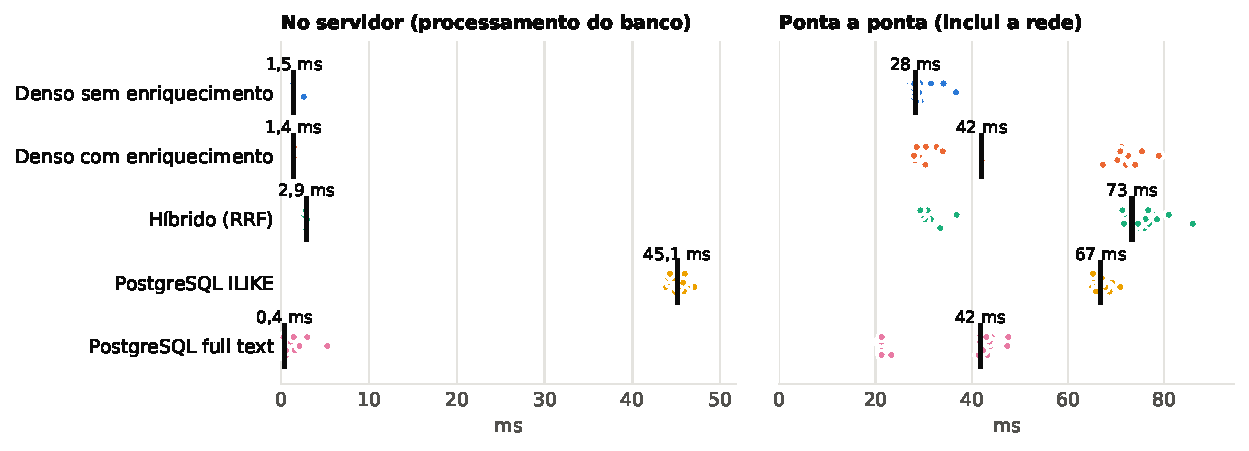
\includegraphics[width=\textwidth]{figuras/fig4-tempo-de-resposta.pdf}
  \fonte{Elaborada pelos autores. Cada ponto é a mediana de cinco repetições de uma consulta; o traço preto é a mediana do motor.}
\end{figure}

O tempo ponta a ponta é dominado pela rede até os clusters em São Paulo e não reflete o custo dos motores. A ida e volta mínima até o Qdrant foi de cerca de 25 ms. As respostas maiores pagam o atraso fixo de cerca de 40 ms já descrito, o que explica os dois grupos visíveis no denso enriquecido e no híbrido. Na busca textual, os dois grupos têm outra causa: as consultas que precisaram ser relaxadas de E para OU fazem duas idas ao banco, e por isso ficam em torno do dobro do tempo das demais. Esse é um custo real do motor, não um efeito de medição. Com a base de 11 mil registros, todos os motores respondem bem abaixo do limite perceptível em uma interface interativa; a diferença de desempenho só se tornaria relevante em volumes muito maiores, em que a busca exaustiva deixa de ser viável e o índice HNSW mostra sua vantagem.

\section{Vantagens e limitações de cada abordagem}
\label{sec:vantagens}

\textbf{Revocação contra precisão.} O híbrido acerta mais no top 5 (80\% contra 68\% da busca textual), mas tem precisão menor (0,42 contra 0,64): traz mais acertos junto com mais ruído. A busca textual, quando encontra algo, encontra bem, mas falha por completo nos erros de digitação e em boa parte das consultas que dependem de significado. Para o usuário do Genérico Certo, encontrar o medicamento certo importa mais que ter os cinco primeiros resultados limpos, porque o passo seguinte é a página de comparação, que lista todos os equivalentes por filtro exato. Por isso o site usa o híbrido como padrão, e a escolha do motor fica disponível apenas na página de comparativo.

\textbf{Sobreposição lexical.} Nas consultas coloquiais, a busca textual empatou com o híbrido. Parte desse resultado se deve à sobreposição de palavras entre as consultas e os termos do dicionário, medida na Tabela~\ref{tab:consultas}: o enriquecimento, aplicado aos dois bancos para manter a comparação justa, também dá à busca textual palavras para casar. Sem o dicionário, as consultas coloquiais seriam quase inacessíveis para as abordagens relacionais, como mostra o \campo{ILIKE}, que exige todas as palavras e não acertou nenhuma.

\textbf{Normalização da camada lexical.} O peso $1/\sqrt{n}$, introduzido para impedir que textos longos dominassem os resultados, tem o efeito oposto de favorecer textos curtos. Nas consultas ``loratadna'' e ``simvastatina'', o ramo lexical colocou a olopatadina e a nistatina, de textos curtos, à frente da loratadina, que aparece só na 7ª posição, e da sinvastatina, cujos registros têm muitos termos populares. Pelo protocolo, esse comportamento não foi ajustado depois de observado nas consultas de teste; fica como limitação declarada e como ponto de melhoria, por exemplo com uma normalização por comprimento do tipo BM25.

\textbf{Busca densa pura.} O modelo multilíngue pequeno representa bem frases descritivas, mas não nomes comerciais nem palavras isoladas raras, e não interpreta negação. O enriquecimento resolve parte das consultas coloquiais, ao custo de depender de conhecimento externo curado manualmente.

\textbf{Abordagem relacional.} O PostgreSQL é imbatível em consultas literais, com resultados limpos e baixo custo, e a busca textual com radicais e relaxamento é uma linha de base forte. Suas limitações são a ausência de tolerância a erros de digitação e a dependência total do vocabulário presente no texto.

\textbf{Reordenação posterior ao benchmark.} A reordenação descrita na Seção~\ref{sec:reordenacao} foi criada depois do benchmark, a partir de uma consulta fora do conjunto de teste, e por isso não altera os resultados oficiais. Para verificar que ela não piora o motor, o híbrido foi medido com e sem ela nas mesmas 25 consultas (\campo{scripts/05-avaliar-reordenacao.ts}). O acerto no top 5 passou de 80\% para 88\%, o MRR@10 de 0,66 para 0,79 e a precisão no top 5 de 0,42 para 0,66. Os ganhos vieram das consultas que citam nome ou apresentação: em ``losartana 50 mg'' o primeiro resultado correto subiu da 6ª para a 1ª posição, e em ``dipirona gotas genérico'', da 8ª para a 1ª. Houve uma piora: em ``dorflex'', o primeiro resultado correto caiu da 1ª para a 3ª posição. A regra do nome sobe todos os produtos com ``dorflex'' no nome, inclusive o Dorflex DIP e o Dorflex UNO, que só têm dipirona e não atendem ao gabarito (a associação de dipirona, orfenadrina e cafeína), e com isso o similar Doricin, equivalente de verdade mas sem a palavra no nome, desceu para fora do top 5. Esses números devem ser lidos com cautela, porque a regra foi desenhada pelo grupo depois de conhecer o comportamento do motor, ainda que sem olhar as consultas de teste; servem como verificação de que a reordenação não prejudica o motor, e não como um novo resultado do experimento. A exceção das vacinas, acrescentada depois, não mudou nenhum desses números.

\textbf{Custo de armazenamento do modelo local.} Rodar o modelo de embeddings dentro da aplicação, em vez de chamar uma API externa, tem custo de armazenamento, e não só de latência. Na Vercel, cada função que carrega o modelo ocupa 342 MB. Na primeira versão publicada, quatro funções o carregavam (as páginas de busca e de comparativo e as rotas de API correspondentes), e cada publicação somava cerca de 2,75 GB nas contas da plataforma; depois de quatro publicações, o time atingiu o limite de 10 GB de armazenamento de funções do plano gratuito. A solução adotada foi concentrar o modelo numa única rota, \campo{/api/embedding}, que recebe o texto da consulta e devolve o vetor; as outras quatro funções pedem o vetor a ela. O custo é uma chamada HTTP interna a mais por busca. A estimativa inicial era de 10 a 30 ms na mesma região; medido em produção, com as funções ativas, gerar o vetor levou cerca de 5 ms dentro da rota de embedding e cerca de 35 ms vistos pela rota de busca (mediana de 25 consultas), ou seja, cerca de 30 ms a mais por busca, com picos ocasionais de 0,7 s quando a plataforma cria uma nova instância da rota de embedding. Em troca, cada publicação passou a ocupar cerca de 0,7 GB, um quarto do anterior. A alternativa descartada foi retirar o modelo do pacote e baixá-lo para o diretório temporário da função na primeira execução: o pacote ficaria pequeno, mas cada instância nova baixaria cerca de 130 MB, o que levaria a partida a frio de 3,7 s para algo entre 5 e 7 s e faria o site depender de o repositório do modelo estar no ar. A abordagem relacional não tem nada disso: as funções que consultam o PostgreSQL ocupam cerca de 2 MB, porque todo o processamento da busca textual acontece dentro do banco, sem modelo, sem binário nativo e sem custo de carregamento.

\textbf{Preço máximo como medida de economia.} A economia mostrada no site compara preços máximos ao consumidor da CMED, que são tetos legais e não preços de balcão. A comparação é correta para o que mede, mas não prevê quanto a pessoa paga, porque cada laboratório dá um desconto diferente sobre o teto. Uma consulta feita pelo grupo em uma grande rede de farmácias em 20/10/2026, para dipirona 1 g com 10 comprimidos, ilustra a diferença. Pelo preço máximo, o Atroveran DIP sai 3\% mais barato que o Dorflex DIP, e a dipirona genérica da Brainfarma (Neo Química), com teto de R\$ 27,30, aparece como mais cara que o Dorflex, de R\$ 17,64. Na farmácia, o Dorflex custava R\$ 15,49 (3\% de desconto), o Atroveran R\$ 12,90 (17\% mais barato que o Dorflex) e a genérica da Neo Química R\$ 11,19 (54\% de desconto sobre o preço de referência da loja e 28\% mais barata que o Dorflex), a mais barata das três. Ou seja, a ordem pelo teto pode se inverter na prateleira, principalmente nos genéricos, que costumam ter teto alto e desconto grande. O grupo considerou mostrar uma faixa de economia (por exemplo, de 12\% a 28\%), mas descartou a ideia: a base não tem nenhuma informação sobre descontos, e uma faixa tirada de uma farmácia, em um dia e para um produto, não valeria para os demais registros. A solução adotada foi rotular a porcentagem como ``no preço máximo'' e avisar, acima da lista de equivalentes, que os descontos variam por laboratório e podem mudar a ordem. Integrar preços reais de farmácias resolveria a limitação, mas não há fonte pública desses preços, e coletá-los dos sites das redes foge ao escopo do trabalho.

\textbf{Limitações do experimento.} O conjunto de teste é pequeno (25 consultas novas, entre 1 e 9 por categoria), o gabarito foi definido pelo próprio grupo, e uma mesma pessoa pode ter escrito o dicionário e as consultas, ainda que em momentos separados pelo congelamento. Os resultados devem ser lidos como indicativos, não como uma avaliação definitiva.

% ---------------------------------------------------------------- 7
\chapter{Conclusão}

O trabalho mostrou que um banco de dados vetorial resolve o problema de vocabulário na busca por medicamentos, desde que a representação vetorial seja pensada para o problema. A busca densa pura, sozinha, foi a pior entre as cinco abordagens avaliadas, com 28\% de acerto no top 5, porque o modelo não representa nomes comerciais nem conhece, a partir dos dados da CMED, para que serve cada medicamento. Duas decisões de modelagem mudaram esse quadro: o enriquecimento do texto com um dicionário de termos populares e a combinação, no próprio Qdrant, de um vetor denso com um vetor esparso de trigramas, fundidos por RRF. Com elas, o acerto chegou a 80\%, à frente da busca textual completa do PostgreSQL (68\%) e do \campo{ILIKE} (36\%), e o motor híbrido foi o único que tratou bem, ao mesmo tempo, nomes comerciais, erros de digitação e linguagem coloquial.

A abordagem relacional se mostrou mais precisa nas consultas literais e mais rápida no servidor, o que reforça que os dois paradigmas são complementares. O ganho do banco vetorial está na revocação e na tolerância a variações de escrita e de vocabulário, que são exatamente as necessidades do usuário leigo. O experimento também evidenciou limitações que permanecem, como a incapacidade dos três tipos de motor de interpretar negação. O uso do site depois do benchmark mostrou ainda que a fusão por posições se beneficia de uma reordenação simples pelo que a consulta pede de forma explícita (nome, dose e quantidade), e que erros de equivalência só aparecem com casos reais, o que levou à tabela de sinônimos de substâncias e à auditoria automática dos grupos de equivalência.

Do ponto de vista metodológico, o trabalho registrou três lições. A primeira é que o conhecimento externo usado para enriquecer os dados pode vazar o gabarito, o que exigiu revisar e congelar o dicionário antes de escrever as consultas. A segunda é que a fusão por posições produz empates que tornam o resultado não determinístico, corrigidos com um desempate fixo. A terceira é que, em serviços na nuvem, o tempo medido no cliente pode refletir a rede e não o banco, o que tornou necessário registrar o tempo no servidor. A aplicação está publicada em \url{https://generico-certo.vercel.app}, e os scripts do repositório reproduzem todas as etapas, da limpeza da lista da CMED ao benchmark.

Como trabalhos futuros, ficam a avaliação de modelos de embedding maiores ou específicos para recuperação, uma normalização da camada lexical baseada em BM25, uma etapa de reordenação capaz de tratar negação, a ampliação do conjunto de teste com gabaritos definidos por profissionais de farmácia, a atualização automática da base a cada nova edição da lista da CMED e a incorporação de preços praticados nas farmácias, caso surja uma fonte pública desses dados.

% ================================================================ REFERÊNCIAS
\postextual
% As referências não são capítulo numerado: o cabeçalho corrido passa a dizer "Referências".
\makeoddhead{relatorio}{\small\itshape Referências}{}{\small\thepage}
\makeevenhead{relatorio}{\small\itshape Referências}{}{\small\thepage}
\bibliography{referencias}

\end{document}
